At the beginning of this project, several months after the end of Støvnengs project, there were still no signs of the new hardware.
To prevent the project from halting dead in its tracks, a decision was taken to order slightly different hardware.
The significant difference to the original system is reduced size of the FPGA, a Spartan-6 LX45T instead of a Spartan-6 LX150T, which entails around 70\% less available resources.
Luckily, the hardware design can be scaled down to fit the smaller chip by reducing the size of the sblock matrix, allowing for implementation of PCI Express and verification of the complete system in hardware.

\subsection{Spartan-6 SP605 Evaluation Platform}

The Spartan-6 SP605 Evaluation Platform is essentially a board with the Spartan-6 LX45T FPGA wired to every useful peripheral imaginable.
It has connections for PCI Express, ethernet, DVI, USB, flash card, JTAG, LEDs, switches, and more.
However, the only peripherals utilized in this project are PCI Express, JTAG, and System ACE flash.
An overview of the system is shown in \figurename~\ref{fig:sp605}.

\begin{figure}[!ht]
    \centering
    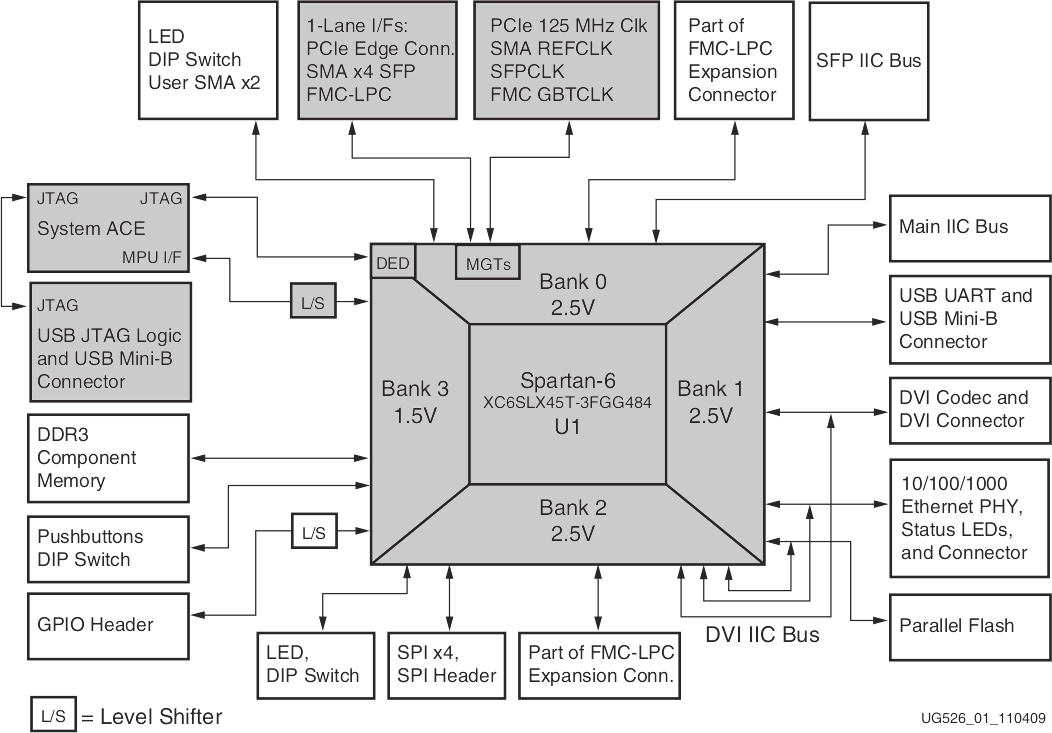
\includegraphics[width=0.48\textwidth]{figures/sp605-modified}
    \caption{High-level block diagram of the SP605 and its peripherals. Parts utilized in this paper are highlighted in gray. (Modified reprint from \cite{ug526})}
    \label{fig:sp605}
\end{figure}

\todo{pci express finger has only data}

\todo{requires external power}

\todo{more?}

\subsection{Hardware setup}

Due to the experimental nature of testing a new hardware platform, two computers were used in this project, as shown in \figurename~\ref{fig:hardware-setup}.
One is the main development workstation, used for coding and synthesis; it has a JTAG connection to the SP605 over USB, which allows it to upload new designs.
The other is the host for the SP605; it is mounted in a PCI Express expansion slot.

\begin{figure}[!ht]
    \centering
    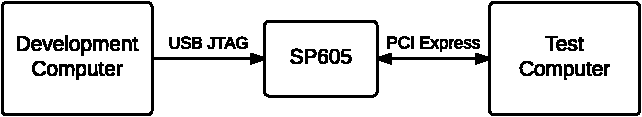
\includegraphics[width=0.40\textwidth]{figures/hardware-setup}
    \caption{High-level block diagram of the hardware setup.}
    \label{fig:hardware-setup}
\end{figure}

The setup allows a new design to be uploaded and tested on the SP605 without the need to reboot the main workstation, due to the power-cycle required to reset the PCI Express connection \CN.

\TODO

\subsection{Software setup}

The operating system on both computers is Linux Mint; version 16 on the development computer and 17 on the test computer.
Linux Mint is currently one of the most popular linux distributions, along with Ubuntu, which it is based upon \cite{distrowatch}.
This means the procedures in this paper should be applicable to most systems.

\todo{USB driver}

\todo{Xilinx ISE 13.3, GCC 4.8.2}

